\documentclass[11pt]{article}

\usepackage{graphicx}
\usepackage{hyperref}

\author{Phan-Anh Nguyen\\
		286049} 
		
\title{Geometry Processing Lab 2012\\
	   Anisotropic Filtering of Non-Linear Surface Features}
	   
\begin{document}
\maketitle



\section{Introduction}

Nowadays, geometric data acquired through imaging or scanning devices has grown rapidly due to advances in technology, making it affordable in many aspects of our lives. However, when dealing with real data we always have to cope with measurement error which brings high frequency noise to our geometric models. Many researches have been conducted in order to remove noise from a scanned model while trying to preserve the underlying sampled surface. One of the seminal results was the work of Taubin et al. \cite{Taubin:1995:SPA:218380.218473} in which they use a signal processing approach to derive the Laplacian operator acting as a low-pass filter on the geometric signal. Even though the Laplacian operator is a powerful tool to remove high frequency noise, it isotropic behaviour makes it unable to preserve sharp features. Hildebrandt and Polthier \cite{Hildebrandt04anisotropicfiltering} have developed an anisotropic method which can preserve high curvature features in a certain direction while suppressing unwanted curvature peaks in the other directions. This method makes it possible to denoise arbitrary surface meshes whereas non-linear geometric features e.g. curved surface regions and feature lines are preserved. This lab report explores and elaborates theory and practice needed to implement the prescribed mean curvature flow proposed by Hildebrandt and Polthier \cite{Hildebrandt04anisotropicfiltering}.

\section{Smoothing Principle}

\begin{figure}[htbp]
  \begin{minipage}[b]{0.45\linewidth}
    \centering
    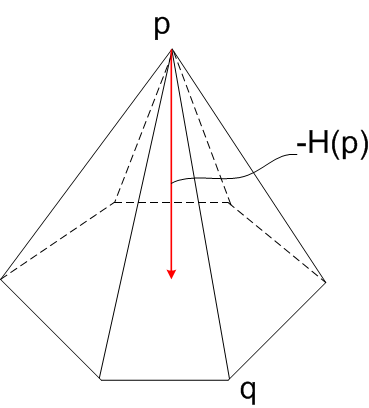
\includegraphics[width=\textwidth]{umbrella.png}
    \caption{smooth a vertex p by moving it in the direction of the mean curvature vector $\vec{H}(p)$}
    \label{fig:umbrella}
  \end{minipage}
  \hspace{0.5cm}
  \begin{minipage}[b]{0.45\linewidth}
    \centering
    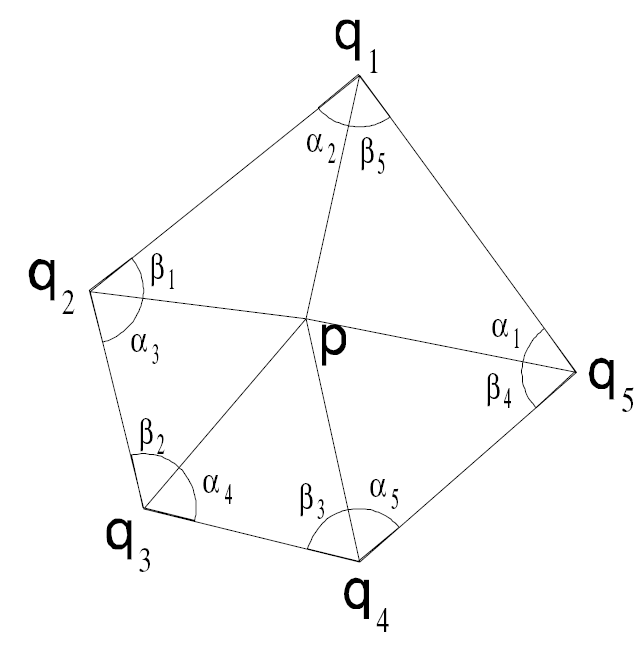
\includegraphics[width=\linewidth]{cotangent.png}
    \caption{Cotangent weights}
    \label{fig:cotangent}
  \end{minipage}
\end{figure}

A very intuitive smoothing operator one can think of is to move a vertex $p$ to the center of gravity (c.o.g) of its one-ring neighbors $N_1(p)$:

\begin{equation}
p \leftarrow \frac{1}{\mid N_1(p) \mid}\sum\limits_{q \in N_1(p)}q = p - \underbrace{\frac{1}{\mid N_1(p) \mid}\sum\limits_{q \in N_1(p)}(p - q)}_{\bigtriangleup p}
\label{eq:update}
\end{equation}

Equation $\ref{eq:update}$ reveals the update form of the smoothing operator in which the old vertex is moved by an amount of the update vector $\bigtriangleup p$ to the new position. The update vector $\bigtriangleup p$ can be generalized to have arbitrary weights over the 1-ring $\sum\limits_{q \in N_1(p)}w_q(p - q)$ other than uniform weights as in the equation $\ref{eq:update}$. In fact, we can choose the weights such that the update vector points in the direction normal to the mesh surface. Such an update formula was first proposed by Pinkall and Polthier \cite{Pinkall93computingdiscrete} known as cotangent weights:

\begin{equation}
\bigtriangledown_p\ area = \vec{H}(p) = 1/2\sum\limits_{q \in N_1(p)}{(cot\alpha_{q} + cot\beta_{q})(p-q)}
\label{eq:cotangent}
\end{equation}

Where $\vec{H}(p)$ is the mean curvature vector at a vertex $p$ and equal the gradient of the area functional $\bigtriangledown_p\ area$ at that vertex. Figure $\ref{fig:umbrella}$ and $\ref{fig:cotangent}$ show how the mean curvature vector is calculated.

\section{Anisotropic Mean Curvature}

The first step toward the formulation of the anisotropic mean curvature vector is to define an edge based mean curvature vector. Given the configuration in figure $\ref{fig:curvature}$ we can easily identify the 2 principal curvature directions $d_{min}$ and $d_{max}$. The minimal curvature direction runs along the common edge $e$ and the maximal one is orthogonal to the plane formed by the edge $e$ and the edge normal vector $n_e = \frac{n_1 + n_2}{\parallel n_1 + n_2 \parallel}$. Obviously the curvature value along the edge $e$ is always zero and the maximal curvature is proportional to the dihedral angle 

\begin{figure}[htbp]
  \begin{minipage}[b]{0.45\linewidth}
	\centering
	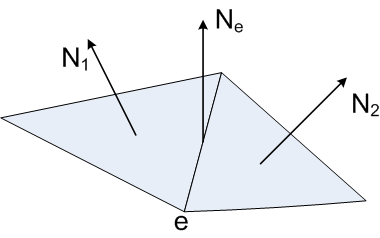
\includegraphics[width=\textwidth]{curvature.png}
	\caption{Edge based mean curvature}
	\label{fig:curvature}
  \end{minipage}
  \hspace{0.5cm}
  \begin{minipage}[b]{0.45\linewidth}
    \centering
    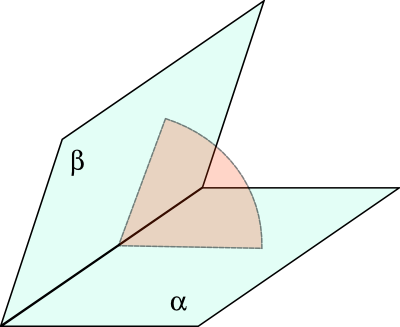
\includegraphics[width=\linewidth]{Dihedral_angle.png}
    \caption{Dihedral angle $\theta_e$}
    \label{fig:dihedral}
  \end{minipage}
\end{figure}

\section{Prescribed Mean Curvature}

Explain volume gradient in detail.

\section{Implementation and Results}

Matrix form: Ha, Mass (non-diagonal converges better => larger time step), Taylor for implicit attempt.

\section{Conclusion and Future Work}



\bibliographystyle{alpha}	% (uses file "plain.bst")
\bibliography{bibliography}		% expects file "myrefs.bib"
\end{document}